\section{Fundamento teórico}

Para comenzar se deben establecer unos parámetros para con la pala, ya que lo más básico de este trabajo empieza por determinar los efectos que produce la torsión en nuestra obtención de energía.

Es por ello que se determina que la pala de la turbina eólica es un \textbf{trapecio} cuya representación simplificada la vemos en la Figura \ref{fig:pala_simp}

\begin{figure}[H]
    \centering
    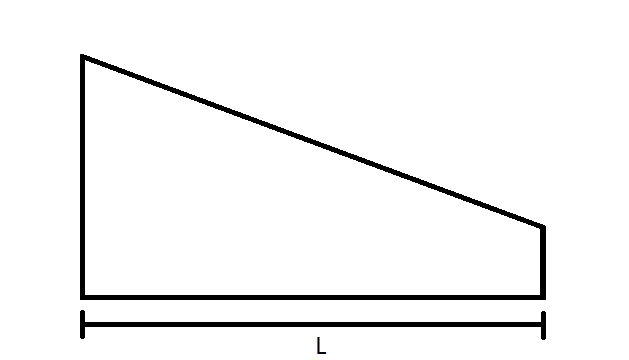
\includegraphics[width=0.7\textwidth]{images/pala turbina paint.png}
    \caption{Representación de una pala de turbina eólica}
    \textit{Fuente: Elaboración propia}
    \label{fig:pala_simp}
\end{figure}

%FALTA POR PONER EL CÁLCULO DEL ÁREA DE LA PALA DEBAJO DE ESTA FIGURA, PARA NO SOLO TENER EL DEL ÁREA DE LOS SEGMENTOS

Lo siguiente que se debe tener presente es que se necesita también una representación de la pala de la figura \ref{fig:pala_simp} dividida en segmentos de igual largo para poder comprender el desarrollo que se realizará simulando una torsión, en la cual se girarán los segmentos un cierto ángulo los unos de los otros.

    \textbf{}
    \begin{figure}[H]
    \centering
    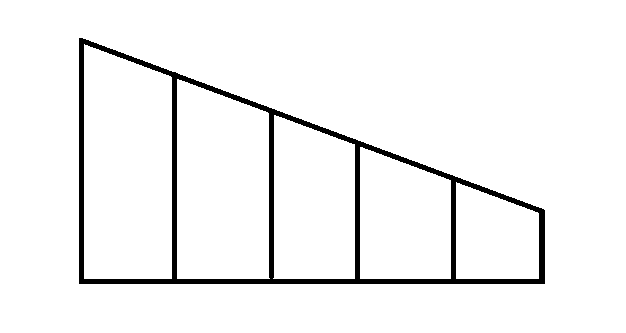
\includegraphics[width=0.7\textwidth]{images/pala dividida.png}
    \caption{Representación de una pala de turbina eólica en segmentos}
    \textit{Fuente: Elaboración propia}
    \label{fig:pala_dividida}
\end{figure}

Por simplicidad, la pala se dividirá únicamente en $N$ segmentos, en este caso 5. Aunque se mantenga este valor durante el trabajo y es probable que no cambie, se asociará a una variable en caso de que se quieran hacer pruebas mediante simulación en MATLAB más adelante. \\\\
    

La $L$ o \textit{longitud de pala}, vista en la Figura \ref{fig:pala_simp} es con la que se va a trabajar, por ello cada uno de los segmentos de la Figura \ref{fig:pala_dividida} tendrá el siguiente largo $\dfrac{L}{N} = \dfrac{L}{5}$ ya que se dividió $N$ número de veces. \\


%SUJETO A CAMBIOS, DEPENDE DE LA RESPUESTA AL CORREO
Como se puede observar en la Figura \ref{fig:pala_dividida} cada segmento tiene una altura variable, esto se debe a la forma real de las palas, cuanto más cerca de la turbina mayor es el tamaño del segmento. \\\\

%SUJETO A CAMBIOS, DEPENDE DE LA RESPUESTA AL CORREO
La altura de estos segmentos depende del valor de una variable, conocida como longitud de cuerda, $c$, que varía dependiendo del segmento en base a un ángulo $\varPhi$, cuanto más alejado del rotor menor será su valor. \\


%FÓRMULA ERRÓNEA, NO SE PUEDE CALCULAR ASÍ EL ÁREA
\begin{definicion}
Se determina el área de los segmentos:
$$ área \text{ } segmento_{i} = \dfrac{L \cdot c_i}{N} $$
donde:
$$ i \in segmento $$
$$ segmento = \{1, ..., N\}$$
\end{definicion}

%SUJETO A CAMBIOS, DEPENDE DE LA RESPUESTA AL CORREO
A continuación, se supone que los segmentos están ensartados por una línea imaginaria que ayudará al estudio de la torsión mediante giros de los segmentos alrededor suya.


\subsection{Estudio del torque con giro inicial}
\label{section:torque_giro_inicial}

Se han presentado algunos de los conceptos básicos, ahora se introduce el ángulo $ \theta_1 $, que es la constante definida como el \textit{giro inicial} que sufrirán todos y cada uno de los segmentos que son paralelos al plano horizontal, desde el cual se presenta el viento que incidirá en nuestra pala.\\

En esta primera sección se estudiará qué ocurre en término de fuerzas, torque y momento cuando se gira toda nuestra pala únicamente el ángulo de giro inicial $ \theta_1 $, sin necesidad de segmentarla, tal y como se aprecia en la figura \ref{fig:pala_simp}. \\


Es cierto que se podría no girar la pala este giro inicial $ \theta_1 $, pero por comodidad de cálculo y para establecer un ángulo de ataque del viento paralelo a la horizontal se realizará de esta manera.\\


Al haber inclinado todos los segmentos un ángulo $ \theta_1 $ se genera la situación en la que el viento incide en el centro del segmento con el mismo ángulo con el que se inclina la pala. \\

    \textbf{}
    \begin{figure}[H]
    \centering
    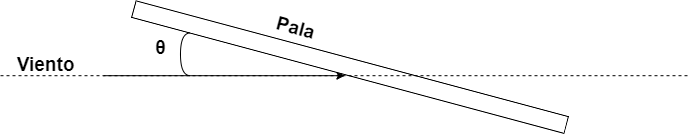
\includegraphics[width=0.8\textwidth]{images/dibujo angulo ataque.drawio.png}
    \caption{Ángulo de ataque del viento con respecto a la pala}
    \textit{Fuente: Elaboración propia}
    \label{fig:dibujo_angulo_ataque}
\end{figure}

La fuerza del viento que incide en la pala se puede descomponer en 2, la tangencial y la normal. \\

    \textbf{}
    \begin{figure}[H]
    \centering
    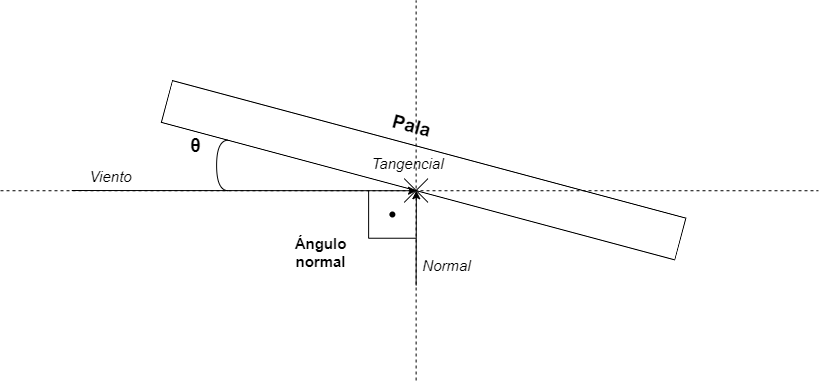
\includegraphics[width=1\textwidth]{images/dibujo fuerzas.drawio.png}
    \caption{Descomposición de vectores de fuerzas}
    \textit{Fuente: Elaboración propia}
    \label{fig:dibujo_fuerzas}
\end{figure}


Como se puede ver en la figura \ref{fig:dibujo_fuerzas} el vector fuerza normal es perpendicular al ángulo de ataque del viento, mientras que el vector fuerza tangencial recorre de manera paralela la línea central de la pala.

 \begin{definicion}
 La fuerza normal genera un ángulo definido por:
 $$ ángulo \text{ } normal = \dfrac{\pi}{2} - \theta_1 $$
 
 \end{definicion}

 \begin{definicion}
 La fuerza normal viene definida por la siguiente expresión:
  $$ f \text{ } normal = F \text{ } viento \cdot \sin{\theta_1}$$
   La fuerza $F \text{ } viento$ será explicada más adelante.
  \label{def:fuerza_normal_inicial}
 \end{definicion}
 
  La componente paralela a la pala, que se ha definido como tangencial se obviará debido a que no genera momento de TORSIÓN (o giro o que) o torque. 
  
  \begin{definicion}
El momento de giro o torque se define como:
 $$ torque_0 = F \text{ } perpendicular \times brazo \text{ } inicial$$
 \label{def:torque_inicial}
 Brazo inicial := distancia entre el inicio de la pala y su centro geométrico. \\
 \end{definicion}
 

     \textbf{}
    \begin{figure}[H]
    \centering
    \includegraphics[width=1\textwidth]{images/explicación brazo inicial.drawio.png}
    \caption{Representación gráfica del brazo de la pala}
    \label{fig:exp_brazo_inicial}
    \textit{Fuente: Elaboración propia}
\end{figure}
 %PUEDE QUE LA IMAGEN ESTÉ MAL, YA QUE CREO QUE SE DEBE TENER EN CUENTA EL ÁNGULO INICIAL Y QUE EL BRAZO VAYA AL CENTRO GEOMÉTRICO DE LA IMAGEN, DESCONOZCO POR AHORA.
 

Para entender visualmente qué es el $brazo \text{ } inicial$ se ha realizado la figura \ref{fig:exp_brazo_inicial}. Ahora es posible pasar a definirlo.

\begin{definicion}
El  brazo inicial viene definido por la siguiente fórmula:
$$ brazo \text{ } inicial = \dfrac{L}{2}$$
\end{definicion}
 
 En la Definición \ref{def:torque_inicial} se encuentra un producto vectorial entre la $fuerza  \text{ }perpendicular \text{ } o \text{ } normal$ y el $brazo$. Pero estas dos variables son perpendiculares la una a la otra. Esto se puede ver ya que $brazo \text{ } inicial$ es completamente paralelo a la $fuerza \text{ } tangencial$. Esto demuestra la perpendicularidad y hace que la Definición \ref{def:torque_inicial} que contenía un producto vectorial de dos parámetros perpendiculares sea definitivamente un producto algebraico, dando lugar a:
 
  \begin{definicion}
  El torque termina siendo un producto algebraico.
 $$ torque_0 = f \text{ } normal \cdot brazo \text{ } inicial$$
 \label{def:torque_algebraico_inicial}
 \end{definicion}
 
   \begin{definicion}
Debido a la geometría de la pala y el brazo inicial, no es necesario el cálculo de un torque global, ya se obtiene con el cálculo natural del propio torque, es por ello que:
 $$ torque \text{ } global_0 = torque$$
 \label{def:torque_global_inicial}
 \end{definicion}
 
 
 Ahora se introduce otro concepto, se trata de la \textit{fuerza del viento}. Gracias a este parámetro, se podrá conocer la fuerza normal que se está produciendo en toda la pala mediante la definición \ref{def:fuerza_normal_inicial}.
 
 \begin{definicion}
 La fuerza del viento para la pala viene dada por:
 
 $$ F \text{ } viento = \dfrac{1}{2} \text{ } \rho \cdot a \cdot u^2$$
 donde:
 
  \centering  $\rho = 1.225 \text{ } \dfrac{Kg}{m^3}$, $a$ := área de la pala, $u$ := velocidad del viento.
 \label{def:fuerza_viento_inicial}
 \end{definicion}
 
 
 
 ...\vspace{400}
 











...
\subsection{Estudio del torque con giro inicial y torsión de la pala}
\label{section:torque_giro_torsion}


\begin{definicion}
Dados el ángulo inicial de giro $\theta_1 $ y una variación de giro constante (o no) $\Delta_\theta$ se define el ángulo de torsión de cada segmento como:
$$\theta_i = \theta_{i-1} + \Delta_\theta$$ 

    donde:
 $$i \in segmento \wedge (i > 1)$$
 
\label{def:theta_cte}
\end{definicion}



\begin{definicion}
Como se menciona, la variación $\Delta_\theta$ puede que no sea constante por conveniencia a la hora de calcular resultados futuros, por ello la definición también puede darse de la siguiente forma:
$$\theta_i = \theta_{i-1} + \Delta_{\theta_{i}}$$ 

    donde:
 $$i \in segmento \wedge (i > 1)$$
\label{def:theta_nocte}
\end{definicion}


La fuerza del viento que incide en la pala se puede descomponer en 2, la tangencial y la normal. \\

 INSERTAR DIBUJO DE LAS FUERZAS \\
 
 \begin{definicion}
 La fuerza normal genera un ángulo de:
 $$ ángulo \text{ } normal_i = \dfrac{\pi}{2} - \theta_i $$
 donde:
 $$ i \in segmento$$
 \end{definicion}

 \begin{definicion}
  Su fuerza se define como:
  $$ f \text{ } normal_i = F \text{ } viento_i \cdot \sin{\theta_i}$$
   donde:
 $$ i \in segmento$$
   \textit{La fuerza $F \text{ } viento_i$ será explicada más adelante.}
  \label{def:fuerza_normal}
 \end{definicion}

 
 La componente paralela a la pala, que se ha definido como tangencial se obviará debido a que no genera momento de TORSIÓN (o giro o que) o torque. 
 
 
 
 \begin{definicion}
El momento de giro o torque se define como:
 $$ torque_i = F \text{ } perpendicular_i \times brazo_i$$
 $$ i \in segmento$$
 \label{def:torque} %para poder referenciarlo fuera
 \textcolor{red}{Brazo := distancia entre el inicio de la pala y el centro del segmento, o radio del segmento.} \\
 \end{definicion}

 La mejor forma de comprender qué se entiende por brazo es mediante la Figura \ref{fig:exp_brazo} en la cual se señalan los segmentos de la pala en distintos colores.
 
     \textbf{}
    \begin{figure}[H]
    \centering
    \includegraphics[width=1\textwidth]{images/explicación brazo.png}
    \caption{Representación gráfica del brazo de la pala}
    \label{fig:exp_brazo}
    \textit{Fuente: Elaboración propia}
\end{figure}

Ahora que visualmente se conoce qué se define por $brazo$, podemos pasar a definirlo.

\begin{definicion}
El  brazo o radio de un segmento $i$ viene definido por la siguiente fórmula:
$$ brazo_i  =  i \cdot \dfrac{L}{2 \cdot N}$$
    donde:
 $$ i \in segmento$$

\end{definicion}

 
 En la Definición \ref{def:torque} se encuentra un producto vectorial entre la $fuerza  \text{ }perpendicular \text{ } o \text{ } normal$ y el $brazo$. Pero estas dos variables son perpendiculares la una a la otra. Esto se puede ver ya que $brazo$ es completamente paralelo a la $fuerza \text{ } tangencial$. Esto demuestra la perpendicularidad y hace que la Definición \ref{def:torque} que contenía un producto vectorial de dos parámetros perpendiculares sea definitivamente un producto algebraico, dando lugar a:
 
  \begin{definicion}
  El torque termina siendo un producto vectorial.
 $$ torque_i = f \text{ } normal_i \cdot brazo_i$$
 $$ i \in segmento$$
 \label{def:torque_vectorial}
 \end{definicion}
 
\begin{definicion}
 La suma de los torques con un giro inicial se conoce como torque global.
 $$ torque \text{ } global_1 \text{ } = \sum_{i=1}^{N} torque_i $$
 donde:
 $$ i \in segmento$$
 \label{def:torque_global}
\end{definicion}


 Ahora se introduce otro concepto, se trata de la fuerza del viento. Gracias a este parámetro, podremos conocer la fuerza normal que se está produciendo en cada uno de los segmentos mediante la definición \ref{def:fuerza_normal}, ya que la fuerza $F$ es su equivalente.
 
 \begin{definicion}
 La fuerza del viento para un segmento viene definida por:
 
 $$ F \text{ } viento_i = \dfrac{1}{2} \text{ } \rho \cdot a_i \cdot u^2$$
 donde:
 
  \centering $i \in segmento$,  $\rho = 1.225 \text{ } \dfrac{Kg}{m^3}$, $a$ := área del segmento i y \\ $u$ := velocidad del viento.
 \label{def:fuerza_viento}
 \end{definicion}
 
 
 \subsubsection{Cálculo de la potencia del sistema}
 
 Una vez se tiene todo lo necesario para el cálculo del torque, se puede pasar al siguiente escalón que sería la potencia. Esta es una unidad de medida que permitirá conocer si el estudio que se está realizando está siendo fructífero, cuanta mayor cantidad de energía se genere, mejor.
 
  \begin{definicion}
 La potencia del sistema con un giro inicial se define como:
 $$ potencia_0 = torque \text{ } global_0 \cdot \Omega_0 $$ 
 
 donde:
 
  \centering $\Omega$ := velocidad de giro o angular de la pala.
 \label{def:potencia_giro_inicial}
 \end{definicion}
 
   \begin{definicion}
 La potencia del sistema con un giro inicial y torsión se define como:
 $$ potencia_1 = torque \text{ } global_1 \cdot \Omega_1 $$ 
 
 donde:
 
  \centering $\Omega$ := velocidad de giro o angular de la pala,\hspace{7} $torque \text{ } global_1$ := Suma de torque de los N segmentos.
 \label{def:potencia_giro_segmentos}
 \end{definicion}
 
 Como se puede observar, se calculó dos veces la potencia, una por cada apartado estudiado. La definición \ref{def:potencia_giro_inicial} corresponde a la sección \ref{section:torque_giro_inicial} que se referencia con un $0$ ya que es la situación inicial y más básica. Mientras que la definición \ref{def:potencia_giro_segmentos} corresponde a la sección \ref{section:torque_giro_torsion} que se ha referenciado con un $1$ ya que nace de la primera.
 
 
 \subsection{Rendimiento de las potencias}
 \label{section:rendimiento}
 
 Una vez se ha realizado la definición de cada una de las fórmulas necesarias para el cálculo de la potencia, se pasa a la comparación de estas. La comparación de potencias nos da como resultado un rendimiento, con este seremos capaces de dictaminar si la torsión de la pala genera una variación en la potencia obtenida.
 
   \begin{definicion}
El rendimiento del sistema viene definido por:
 $$ \eta = \dfrac{potencia_1}{potencia_0} $$ 
 
 donde:
 
  \centering $potencia_0$ := Energía del sistema unicamente con un giro inicial, \hspace{4} $potencia_1$ := Energía del sistema con giro inicial y segmentos torsionados
 \label{def:rendimiento_potencias}
 \end{definicion}
 
 Una vez se ha definido el rendimiento y se calcula en base a los resultados obtenidos mediante asignación de valores a variables estándar y aplicando estos a las definiciones relacionadas, se pueden dar 3 escenarios:
 
  \begin{enumerate}
    \item $\eta < 0$ \label{enum:menor_cero}
    \item $\eta = 0$ \label{enum:igual_cero}
    \item $\eta > 0$ \label{enum:mayor_cero}
\end{enumerate}
 
